\documentclass{beamer}

\usepackage{fontspec,xunicode,xltxtra}

\usepackage{tikz}

\XeTeXlinebreaklocale "zh"
\XeTeXlinebreakskip = 0pt plus 1pt minus 0.1pt

%\setmainfont[Mapping=tex-text]{AR PL UMing CN:style=Light}
%\setmainfont[Mapping=tex-text]{AR PL UKai CN:style=Book}
%\setmainfont[Mapping=tex-text]{WenQuanYi Zen Hei:style=Regular}
%\setmainfont[Mapping=tex-text]{WenQuanYi Zen Hei Sharp:style=Regular}
%\setmainfont[Mapping=tex-text]{AR PL KaitiM GB:style=Regular} 
%\setmainfont[Mapping=tex-text]{AR PL SungtiL GB:style=Regular} 
%\setmainfont[Mapping=tex-text]{WenQuanYi Zen Hei Mono:style=Regular} 

\newfontfamily\hei{WenQuanYi Micro Hei}
\newfontfamily\whei{WenQuanYi Zen Hei}
\newfontfamily\kai{AR PL UKai CN}
\newfontfamily\song{AR PL UMing CN}
\newfontfamily\bhei{cwTeXHeiBold}
%\newfontfamily\lishu{SIMLI}
\setmainfont[Mapping=tex-text]{WenQuanYi Micro Hei}
\setsansfont[Mapping=tex-text]{AR PL UKai CN}
\setmonofont[Mapping=tex-text]{WenQuanYi Zen Hei Mono}

\renewcommand{\baselinestretch}{1.25}


\mode<presentation>
{
  \usetheme{Warsaw}
  % or ...
  %\usetheme{default}

  \setbeamercovered{transparent}
  % or whatever (possibly just delete it)
}


\usepackage[english]{babel}
% or whatever

%\usepackage[latin1]{inputenc}
% or whatever

\title[MS2023] % (optional, use only with long paper titles)
{\Huge 数学软件}

\subtitle
{Math Software} % (optional)

\author[Wang HY] % (optional, use only with lots of authors)
{王何宇}
% - Use the \inst{?} command only if the authors have different
%   affiliation.

\institute[Zhejiang University] % (optional, but mostly needed)
{
  浙江大学数学科学学院\\
  计算数学系
}
% - Use the \inst command only if there are several affiliations.
% - Keep it simple, no one is interested in your street address.

\date[Short Occasion] % (optional)
{}


% If you have a file called "university-logo-filename.xxx", where xxx
% is a graphic format that can be processed by latex or pdflatex,
% resp., then you can add a logo as follows:

\pgfdeclareimage[height=1cm]{university-logo}{images/zju.jpg}
\logo{\pgfuseimage{university-logo}}

% Delete this, if you do not want the table of contents to pop up at
% the beginning of each subsection:
%\AtBeginSubsection[]
%{
%  \begin{frame}<beamer>{Outline}
%    \tableofcontents[currentsection,currentsubsection]
%  \end{frame}
%}


% If you wish to uncover everything in a step-wise fashion, uncomment
% the following command: 

%\beamerdefaultoverlayspecification{<+->}


\begin{document}

\begin{frame}
 \titlepage
\end{frame}
%\begin{frame}{Outline}
%  \tableofcontents
  % You might wish to add the option [pausesections]
%\end{frame}

\begin{frame}{自我介绍}
  \begin{itemize}
  \item 王何宇, 浙江大学数学科学学院, 信息与计算科学系.
  \item email: wangheyu@zju.edu.cn
  \item 手机: 13456940632
  \item 我承担很多信息与计算方向的专业课程, 所以大概率会和大家共事 3 年甚至更多.
  \end{itemize}
\end{frame}

\begin{frame}{使用计算机的基本原则}
  \begin{itemize}
  \item<1-> 用计算机提升你的工作和学习效率,而不是相反;
  \item<2-> 白嫖使人快乐! 
  \item<3-> 参与和回馈社区;
  \item<4-> 如果你是计算数学,应用数学和统计的同学,像重视黑板那样重视计算机;
  \item<5-> 一切都在非线性变化,保持清醒和独立思考,只学对你现实有用的计算机技能。
  \end{itemize}
\end{frame}

\begin{frame}{学习本课的基本条件}
  \begin{itemize}
  \item<1-> 一个可以正常运行的 Linux 系统, 可以是独立系统, 双系统, 云主机, 或虚拟机.
  \item<2-> 能正确使用键盘, 打字速度不宜太低.
  \item<3-> 未来计划走应用数学的发展方向.
  \item<4-> 如果以上条件不能满足, 也不准备克服, 建议立刻退课或换课, 以免浪费时间.
  \end{itemize}
\end{frame}

\begin{frame}{和计算机交流}
  \begin{columns}[c]
% create the column with the first image, that occupies
% half of the slide
    \begin{column}{.5\textwidth}
      \begin{itemize}
      \item<1-> 机器内部使用的是二进制数据流;
      \item<2-> 使用 shell: 打开终端,输入命令,得到反馈;
      \item<3-> 阅读和实现: Beginning Linux Programming 4th edtion, chapter 2.
      \item<4-> 通过脚本实现自动化操作.
      \end{itemize}
    \end{column}
% create the column with the second image, that also
% occupies half of the slide
    \begin{column}{.5\textwidth}
    \begin{figure}
        \centering
        \includegraphics<1>[width=0.75\textwidth]{../images/matrix.bmp}
        \includegraphics<1>[width=0.75\textwidth]{../images/blank.png}       
        \includegraphics<2->[width=0.75\textwidth]{../images/matrixbin.png}
        \includegraphics<2->[width=0.75\textwidth]{../images/shell.png}
    \end{figure}
    \end{column}
\end{columns}
  %% \begin{tikzpicture}
  %%   \node (img1) {\includegraphics[height=3cm]{res/matrix.bmp}};
  %% \end{tikzpicture}
\end{frame}

\begin{frame}{文本编辑器}
  \begin{itemize}
  \item<1-> 能基本上完全用键盘控制.
  \item<2-> 适合终端和 shell 的模式, 不占用太多的软硬件和通讯资源.
  \item<3-> 能快速高效地发送和接受指令, 完成编码.
  \item<4-> 推荐: emacs, vim, vscode.
  \item<5-> 选择一款最适合你自己, 能把你的工作效率提到最高的编辑器.
  \item<6-> 如果你不知道怎么配置你的编辑器, 用缺省配置, 或者像同行要一个配置文件. 
  \end{itemize}
\end{frame}

\begin{frame}{科技文献排版}
  \begin{itemize}
  \item<1-> Tex 和 Latex,以及中文化;
  \item<2-> 编辑器的选择:vscode,vim 或 emacs;
  \item<3-> 从源代码到 pdf,文稿和 slide;
  \item<4-> 点阵图和矢量图;
  \item<5-> 文献管理;
  \end{itemize}
\end{frame}

\begin{frame}{如何产生漂亮的数学文章}
  \begin{tikzpicture}[remember picture, overlay]
    \node[left = 2cm, above = -0.1cm] at (current page.east) 
         {
           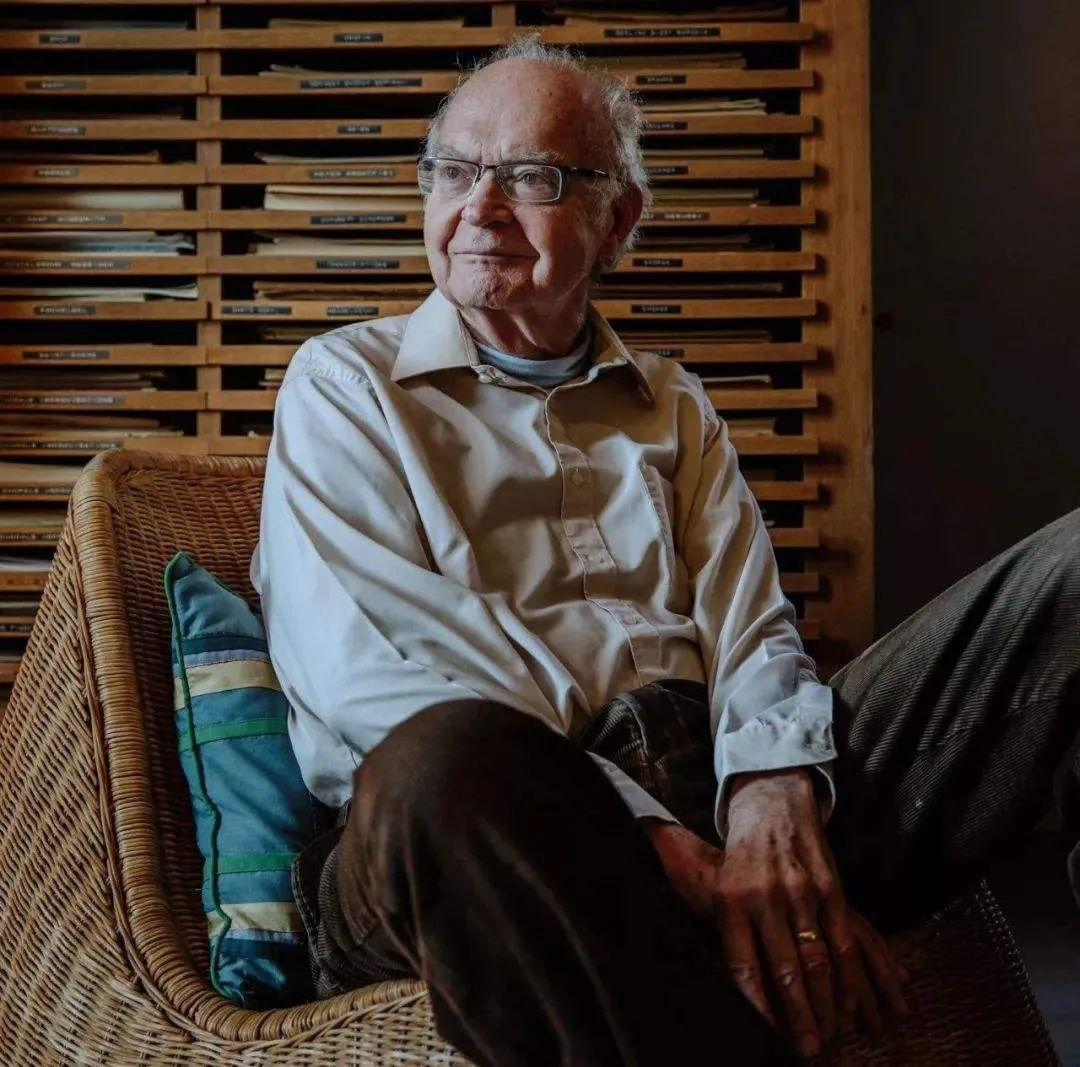
\includegraphics[width=0.25\textwidth]{../images/knuth.png}
         };
\end{tikzpicture}  
  \begin{itemize}
  \item<1-> 数学家对写作有特殊的要求.
  \item<2-> 同样必须满足键盘, 终端和高效的原则.
  \item<3-> 唯一解也是事实上的标准: \LaTeX.
  \item<4-> 参考资料: lshort, manual, ...
  \item<5-> 去找一个例子.
  \item<6-> 必须亲自动手写点什么. 
  \end{itemize}
\end{frame}

\begin{frame}{编译和项目管理}
  \begin{itemize}
  \item<1-> 自动编译:make 和 cmake;
  \item<2-> 数据保存:云盘和 git;
  \item<3-> 进入开源社区:github 和 gitee;
  \item<4-> 项目实践;
  \end{itemize}
\end{frame}

\begin{frame}{C/C++ 和 Linux 系统}
  \begin{itemize}
  \item<1-> 编译器:gcc 和 icc;
  \item<2-> C 和 C++ 简介;
  \item<3-> 可执行文件,头文件和类库;
  \item<4-> 命令行和管道;
  \item<5-> C / C++ 的自动化编译和部署;
  \end{itemize}
\end{frame}

\begin{frame}{计算软件}
  \begin{itemize}
  \item<1-> 基础数学库:blas,lapack 和 gsl;
  \item<2-> 专用计算库:eigen,deal.ii; 
  \item<3-> 通用计算软件:matlab,octave 和 北太天元;
  \item<4-> 可视化工具:paraview;
  \item<5-> 一切皆可使用:python,chatGPT,...
  \end{itemize}
\end{frame}

\end{document}


